\section{Постановка задачи}
%\chapter{Постановка задачи}

\begin{figure}[h]
    \caption{Семантическая и <<объектная>> сегментация \label{fig:semantic_and_instance_segmentation}}
    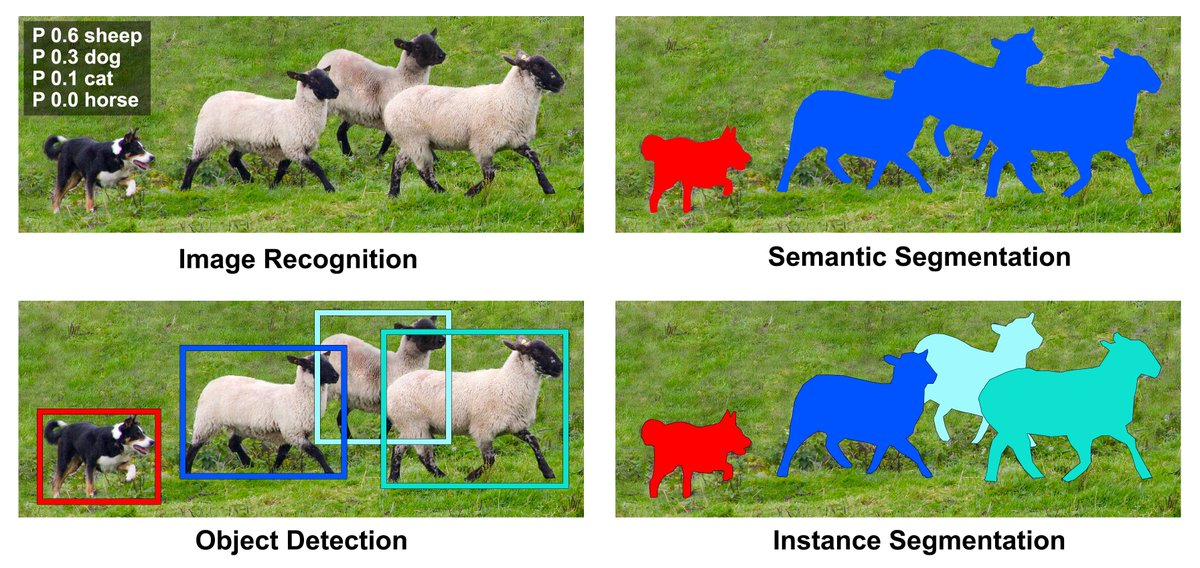
\includegraphics[scale=0.4]{instance_and_semantic_segmentation.jpg}
\end{figure}

Сегментация~--- это задача разбиения изображения на области.
Выделяют семантическую сегментацию и <<объектную>> сегментацию
\footnote{Semantic и Instance segmentation соответственно. Для последней устоявшегося русскоязычного термина нет.}.

При семантической сегментации каждому пикселю сопоставляется класс объекта, в котором он находится.
Пример можно видеть на рис. \ref{fig:semantic_and_instance_segmentation}, в верхнем правом углу.
Следует обратить внимание, что если на изображении есть несколько объектов одного класса, то они все обозначаются одним цветом.

При <<объектной>> сегментации (справа снизу на рис. \ref{fig:semantic_and_instance_segmentation}) требуется не только определять класс, но и отличать разные объекты одного класса.

Потребность в сегментации изображений возникает в медицине, в распознавании лиц, в системах управления беспилотными автомобилями и многих других областях.
Это актуальная задача, имеющая важное прикладное значение.

\subsection*{Обучение с учителем и без учителя}
Задача сегментации сейчас решается методами машинного обучения.
Поэтому для дальнейшего изложения понадобится ввести понятия обучения с учителем и без учителя.

Обучение с учителем (supervised learning)~--- это сеттинг, в котором мы предполагаем, что есть множество объектов $\mathcal{X}$,
множество ответов $\mathcal{Y}$ и существует некоторое неизвестное отображение $f\colon \mathcal{X} \mapsto \mathcal{Y}$.
Нам дана обучающая выборка $\bigl( \mathbb{X}, \mathbb{Y}\bigr) = \{ (x_i, y_i)\colon x_i \in \mathcal{X}, \; y_i \in \mathcal{Y}, \; f(x_i) = y_i, \; i = \overline{1, n}\}$,
и требуется восстановить неизвестное отображение $f$.

В эту парадигму укладываются, например, задачи классификации и регрессии.
В первом случае множество $\mathcal{Y}$ конечно. Можно без ограничения общности считать, что $\mathcal{Y} = \{1, \ldots, K\}$, где $K$ - число классов.
Во втором случае множество $\mathcal{Y}$ бесконечно. Чаще всего $\mathcal{Y} = \mathbb{R}$.

Множество $\mathcal{X}$, как правило, является некоторым подмножеством $\mathbb{R}^d$.
Компоненты вектора $x = (x_1, \ldots, x_d)$ называются признаками.
В некоторых случаях объекты имеют сложную структуру~--- например, если мы рассматриваем графы или временные ряды,
и найти хорошее признаковое описание (т.е., представить объект в виде вектора чисел) само по себе является нетривиальной задачей.
При работе с изображениями, к счастью, есть довольно естественный путь --- использовать его RGB-представление.

При обучении с учителем обычно вводят некоторый параметрический класс функций $\mathcal{F} = \{f_\theta\colon \mathcal{X} \mapsto \mathcal{Y}, \; \theta \in \Theta\}$,
в котором будет искаться решение, {а также функцию потерь $\mathcal{L}$}.

Примерами множества $\mathcal{F}$ могут служить линейные комбинации признаков в случае линейной регрессии, 
кусочно-постоянные функции в случае решающих деревьев или более общие и сложно описываемые классы в случае нейронных сетей.

Функция потерь используется для формализации понятия качества модели $f_\theta \in \mathcal{F}$.
Примерами функций потерь для задачи регрессии могут является среднеквадратичная ошибка и среднее абсолютное отклонение;
для задачи классификации~--- кросс-энтропия.

Процесс обучения заключается в поиске такого $\theta^* \in \Theta$, что $f_{\theta^*}$ наилучшим образом приближает $f$
в смысле минимизации выбранной функции потерь $\mathcal{L}$.

Обучение с учителем удобно тем, что допускает довольно стройное математическое описание, и по существу сводится к оптимизации некоторого функционала.
\medskip

Обучение без учителя (unsupervised learning) описать несколько сложнее.
К нему относят такие задачи, как кластеризация, оценка плотности, понижение размерности, визуализация, поиск аномалий.
Можно сказать, что в этом случае мы имеем некоторый набор данных $\mathbb{X} = \{x_1, \ldots, x_n\}$ объектов из множества $\mathcal{X}$
и пытаемся найти в нём некоторые структурные особенности.
\bigskip

Вернёмся к сегментации. Понятно, что если у нас есть набор картинок, для которых известна правильная разметка, 
то мы можем рассматривать нашу задачу как задачу обучения с учителем. А более конкретно, как классификацию пикселей.
%В этом случае можно добиться хорошего качества, используя свёрточные нейронные сети или архитектуры на основе трансформера.

Однако, специфика сегментации изображений заключается в том, что создание обучающей выборки крайне трудоёмко.
Мы должны сопоставить класс каждому пикселю изображения, а на одной картинке разрешения $1024 \times 1024$ их уже более миллиона.
В то же время для обучения качественной модели требуются, как правило, тысячи изображений.  
Более того, разметка, скажем, медицинских изображений не может быть выполнена случайным человеком~--- требуется привлечение специалиста.

Эти проблемы мотивируют желание интерпретировать сегментацию изображений как задачу обучения без учителя,
или по крайней мере снизить объём размеченных данных, необходимых для обучения.